\section{Empirical Evaluation} \label{Sec:evaluation}
To quantitatively assess the efficacy of our test generation approach, we have conducted a case study, in which we address the following research questions:

\begin{description}
\item [RQ1] How accurate is \atrina in mapping DOM-based assertions to the corresponding \javascript code?
\item [RQ2] How effective is \atrina in generating unit test assertions that detect faults?
\item [RQ3] Is our approach more effective than DOM-based assertions written manually by the tester in terms of fault finding capability? 
\item [RQ4] How does our approach compare to existing mutation-based assertion generation techniques?
\end{description}
%
%\atrina and the experimental data are available for download \cite{atrina-dl}.
\subsection{Objects}
Our study includes four open source \javascript web applications that have \selenium test cases.
%Finding applications with executable Selenium test cases for \javascript applications is a big challenge.
\tabref{objectsTable} presents the experimental objects and their properties. Phormer \cite{phormer} is a photo gallery web application. EnterpriseStore \cite{enterpriseStore} is an asset management web application. WolfCMS \cite{wolfcms} is a content management system, and Claroline \cite{claroline} is a collaborative online learning and course management system. 
\begin{table}
        \caption{Characteristics of the experimental objects.} \label{Table:objectsTable}  
%        \vspace{-0.1in}       
{\scriptsize
\centering
%    \begin{center}
       
      %  \subtable[Experimental subjects and the corresponding exploration data]
            {
           \begin{tabular}{l|l|l|>{\centering}m{1cm}|c} \hline
\thead{ID} &\thead{Name} &\thead{LOC (JS)} &\thead{\# Test Cases} &\thead{\# Assertions}  \\  \hline 

\hline

1  & Phormer & 1.5K & 7 & 18    \\ \hline
           
2 & EnterpriseStore & 57K & 19 & 21  \\ \hline

3 & WolfCMS & 1.3K & 12 & 42  \\ \hline

4 & Claroline & 36K & 23 & 35 \\ \hline

5 & StudyRoom & 10.6K & 12 & 23 \\ \hline

6 & AddressBook & 1.1K & 13 & 14 \\ \hline

7 & Brotherhood & 0.8K & 10 & 10 \\ \hline
\end{tabular}
            }

%\end{center}
}
\vspace{-0.2in} 
\end{table}
\subsection{Setup} \label{Sec:setup}
To address our research questions, we provide the URL as well as the available manually written DOM-based test suite of each experimental object to \atrina. Unit level test assertions are then automatically generated by the tool.
\headbf{Accuracy (RQ1)} To evaluate the accuracy of \atrina, we measure precision and recall. We manually compare the slices generated by \atrina with the \javascript code that is relevant to each assertion. Precision and recall are defined as follows:
\begin{description}[noitemsep, nolistsep, font=\normalfont\itshape]
\item [Precision] is the fraction of lines in a slice produced by \atrina, that are actually related to the human-written DOM-based assertion: $\frac{TP}{TP+FP}$ 
\item [Recall] is the fraction of the correct set of related lines of code to each assertion, which is actually present in the slice produced by \atrina: $\frac{TP}{TP+FN}$ 
\end{description}
where $TP$ (true positives), $FP$ (false positives), and $FN$ (false negatives) respectively represent the number of lines of code that are correctly reported, falsely reported, and missed to report as related to the DOM-based assertion.
\headbf{Effectiveness (RQ2)} To assess the effectiveness of \atrina, we measure the fault finding capability of the assertions generated by the tool. Moreover, to understand the effect of each type of assertion produced by \atrina in detecting faults, we compare the fault detection rate of using (1) exclusively explicit assertions, (2) explicit assertions and implicit assertions, and (3) explicit assertions and candidate assertions. Since explicit assertions compose the core body of our assertions, we consider implicit and candidate assertions in conjunction with explicit ones rather than separate them.
       
The experimental objects do not come with a rich version history to apply \atrina on real regression changes. Therefore we mimic regression faults by automatically injecting mutations to the application, and evaluate the tool's ability in detecting the seeded faults. Using our recently developed mutation testing tool, \mutandis \cite{mirshokraie:icst13}, we automatically inject 50 random first-order mutations into the \javascript code of the applications. The mutation operators are chosen from a list of common operators such as changing the value of a variable, modifying a conditional statement, altering unary operations, as well as common mistakes made by developers when developing a given web application \cite{mirshokraie:tse15}, e.g., changing the ID/tag name passed into DOM access functions such as \code{getElementById} or \code{getElementsByTagName}, and modifying the attribute name/value in \code{setAtt\-ribute}. The fault is considered detected if an assertion generated by \atrina fails when run on the mutated code, and our manual examination confirms that the failed assertion is detecting the seeded fault.
\headbf{Comparison with human-written DOM-based Assertions (RQ3)} To assess the usefulness of \atrina, we compare the human written DOM-based assertions with the unit-level test assertions generated by our approach in terms of fault finding capability.
Similar to RQ2, we perform fault injection on both.
The faults injected into our experimental objects in response to RQ3 are the same as the ones that we seed in applications to answer RQ2.
\headbf{Comparison with Mutation-based Assertion Generation (RQ4)} To assess how \atrina performs with respect to the current state-of-the-art oracle generation technique, we compare our tool's fault finding capability with the mutation-based assertion generation approach \cite{mirshokraie:icst15, fraser:tse12}. To generate mutation-based assertions for the \javascript code, we use human-written DOM-based test suite as a means to execute the application and infer the execution traces required for the purpose of mutation analysis. We perform the following steps to generate test assertions using mutation analysis.
\begin{enumerate}[noitemsep, nolistsep]
\item Remove assertions from the human-written DOM-based test suite.
\item Execute the test suite on the original version of the application to obtain execution traces.
\item Inject mutations for the purpose of oracle generation.
\item Execute the human-written test suite on the generated mutants, and produce test oracles by comparing execution traces obtained from the mutants and the original version of the application.
\end{enumerate}
The number of mutants, that are generated to produce test assertions is 50 for each application. Note that the implementation and evaluation of the mutation analysis technique both use mutation operators from our prior work \cite{mirshokraie:tse15}. Therefore, our evaluation is biased in favour of mutation-based assertion generation approach over our technique.
\subsection{Results} \label{Sec:results}

%\begin{table}
%\vspace{5pt}
        \caption{Code coverage achieved for test cases generated by \tool and \artemis.}
{\scriptsize
    \begin{center}
       
      %  \subtable[Experimental subjects and the corresponding exploration data]
            {
           \begin{tabular}{c|c|c} \hline
\thead{App ID} &\theadturn{\tool (\%)} &\theadturn{\artemis  (\%)}  \\  \hline \hline

1  & 99 &  92 \\ \hline
           
2 & 78 &  49 \\ \hline

3 & 90 & 35 \\ \hline

4 & 75 &  65 \\ \hline

5 & 49 &  15 \\ \hline

6 & 78 &  66 \\ \hline

7 & 63 &  0 %30
 \\ \hline

8 & 56 & 0 % 42
  \\ \hline

9 & 82 &  63 \\ \hline

10 & 71 & 67  \\ \hline

11 & 56 &  46 \\ \hline

AVG& 72.5 & 45.3 \\ \hline


\hline\end{tabular}\centering
            }
\label{Table:covg-table}
\end{center}
}
\end{table} 


%\headbf{Function coverage maximization (RQ1)} \tabref{efficiency-abs-mut-table} presents the statement coverage achieved by using our function coverage maximization technique and the random strategy. Our results show on average 9\% improvement in statement coverage, across all the applications. We observed that our technique achieves the highest improvement when there are dynamically generated clickables in the application.
%
%For example, for Tunnel (ID 2) and Fractal Viewer (ID 9), we observed no improvement in the statement coverage as these two applications have no dynamically generated or bound to event-listeners clickables. Instead, their few clickables are all placed in the HTML code of the application with a fixed event-handler per clikcable. Thus,  our approach achieves the same coverage as the random strategy for such applications.
%
%For SameGame (ID 1) the number of executed functions remains the same, for both approaches. However, in the limited five minute period of time, as a result of dynamically detecting valid clickable elements, \tool is able to examine different paths of the applications, while the random exploration technique fails to do so as it blindly clicks on any candidate element on the DOM tree.
%
%Finally, GhostBusters (ID 3) benefits the most from our dynamic exploration technique. This application contains a large number of dynamically created clickable DOM elements that appear and then disappear within a few seconds. We observed two anonymous functions, attached to clickable elements, that are missed by the random exploration technique in this application. Our technique is not only able to quickly spot such on the fly generated clickables, but it is also able to click on the ones that result in the execution of uncovered functions. 
%These two functions are attached to clickable elements that are not executed using random strategy. 

\begin{table}
\center
%\vspace{5pt}
        \caption{Results showing the effects of our \textbf{function coverage maximization}, \textbf{function state reduction}, and \textbf{mutation-based oracle generation} algorithms.}
        \label{Table:efficiency-abs-mut-table}
{\scriptsize
       
      %  \subtable[Experimental subjects and the corresponding exploration data]
            {
           \begin{tabular}{c|r|r||r|r|r||r|r} \hline
&\multicolumn{2}{c||}{\thead{St. Coverage}} & \multicolumn{3}{c||}{\thead{State Reduction}} & \multicolumn{2}{c}{\thead{Oracles}}\\
\cline{2-8}

\theadturn{App ID} &

\theadturn{Fun. cov. maximize (\%)} & \theadturn{Random exploration (\%)} 
&\theadturn{\#Func.States w/o reduction} &\theadturn{\#Func.States with reduction}  &\theadturn{Func.State Reduction (\%)}
%&\multicolumn{2}{c}{\thead{Assertions}} \\ 
%\cline{5-6}&

&\theadturn{\#Assertions w/o mutation} &\theadturn{\#Assertions with mutation}  \\  \hline

\hline

1 & 99 & 80 & 447 & 42 & 91 & 5101 & 171\\ 

2 & 78 & 78 & 828 & 23 & 97 & 23212 & 91\\ 

3 & 90 & 66 & 422 & 22 & 95 & 3520 & 69 \\ 

4 & 75 & 75 & 43 & 18 & 58 & 1232 & 105\\ 

5 & 49 & 45 & 534 & 31 & 94 & 150 & 103\\ 

6 & 78 & 75 & 797 & 38 & 95 & 1648 & 149\\ 

7 & 63 & 58 & 1653 & 58 & 96 & 198202 & 365\\ 

8 & 56 & 50 & 32 & 23 & 28 & 78 & 67 \\ 

9 & 82 & 82 & 1509 & 51 & 97 & 65403 & 259 \\ 

10 & 71 & 69 & 71 & 22 & 69 & 6584 & 94 \\ 

11 & 56 & 54 & 1383 & 136 & 90 & 2530 & 334 \\ 

12 & 41 & 38 & 1530 & 64 & 96 & 3521 & 193 \\ 

13 & 51 & 47 & 1401 & 161 & 88 & 2481 & 361 \\ \hline

AVG& 68.4 & 62.8 & - & - & 84.1 & - & - \\  \hline
          
\hline\end{tabular}\centering
            }
}
\vspace{-0.18in}
\end{table}


%\begin{table}
%%\vspace{5pt}
%\centering
%        \caption{Results showing the effects of our \textbf{function coverage maximization}, \textbf{function state reduction}, and \textbf{mutation-based oracle generation} algorithms.}
%        \label{Table:efficiency-abs-mut-table}
%{\scriptsize
%       
%      %  \subtable[Experimental subjects and the corresponding exploration data]
%            {
%           \begin{tabular}{c|c|c||c||>{\centering}b{1.3cm}|c||>{\centering}b{1.3cm}|c||c|c} \hline
%&\multicolumn{2}{c||}{\thead{St. Coverage}} 
%& \multirow{3}{*}{\theadturn{\#Function states w/o state removal}} & 
%\multicolumn{2}{c||}{\thead{St. Reduction-Mutation}} & \multicolumn{2}{c||}{\thead{St. Mutation-Reduction}} & \multicolumn{2}{c}{\thead{Oracles}}\\
%\cline{2-3} \cline{5-10}
%
%\theadturn{App ID} &
%
%\theadturn{Fun. cov. maximize (\%)} & \theadturn{Random exploration (\%)} &&\theadturn{\#Func.States using Reduc-Mut }  &\theadturn{Func.State Reduction (\%)}
% &\theadturn{\#Func.States using Mut-Reduc }  &\theadturn{Func.State Reduction (\%)}
%%&\multicolumn{2}{c}{\thead{Assertions}} \\ 
%%\cline{5-6}&
%
%&\theadturn{\#Assertions w/o mutation} &\theadturn{\#Assertions with mutation}  \\
%&&&&&&&&& \\
%  \hline
%
%\hline
%
%1 & 99 & 80 & 447 & 33 & 93 & & & 5101 & 136\\ 
%
%2 & 78 & 78 & 828 & 21 & 97 & & & 23212 & 81\\ 
%
%3 & 90 & 66 & 422 & 14 & 96 & & & 3520 & 45 \\ 
%
%4 & 75 & 75 & 43 & 19 & 56 & & & 1232 & 109\\ 
%
%5 & 49 & 45 & 534 & 23 & 95 & & & 150 & 79\\ 
%
%6 & 78 & 75 & 797 & 30 & 96 & & & 1648 & 125\\ 
%
%7 & 63 & 58 & 1653 & 54 & 97 & & & 198202 & 342\\ 
%
%8 & 56 & 50 & 32 & 18 & 43 & & & 78 & 51 \\ 
%
%9 & 82 & 82 & 1509 & 49 & 97 & & & 65403 & 253 \\ 
%
%10 & 71 & 69 & 71 & 23 & 67 & & & 6584 & 96 \\ 
%
%11 & 56 & 54 & 1383 & 131 & 90 & & & 2530 & 318 \\ 
%
%12 & 41 & 38 & 1530 & 62 & 96 & & & 3521 & 184 \\ 
%
%13 & 51 & 47 & 1401 & 152 & 89 & & & 2481 & 335 \\ \hline
%
%AVG& 68.4 & 62.8 & - & - & 85.5 & & & - & - \\  \hline
%          
%\hline\end{tabular}\centering
%            }
%}
%\vspace{-0.18in}
%\end{table}

\begin{figure}[!t]
  \centering
  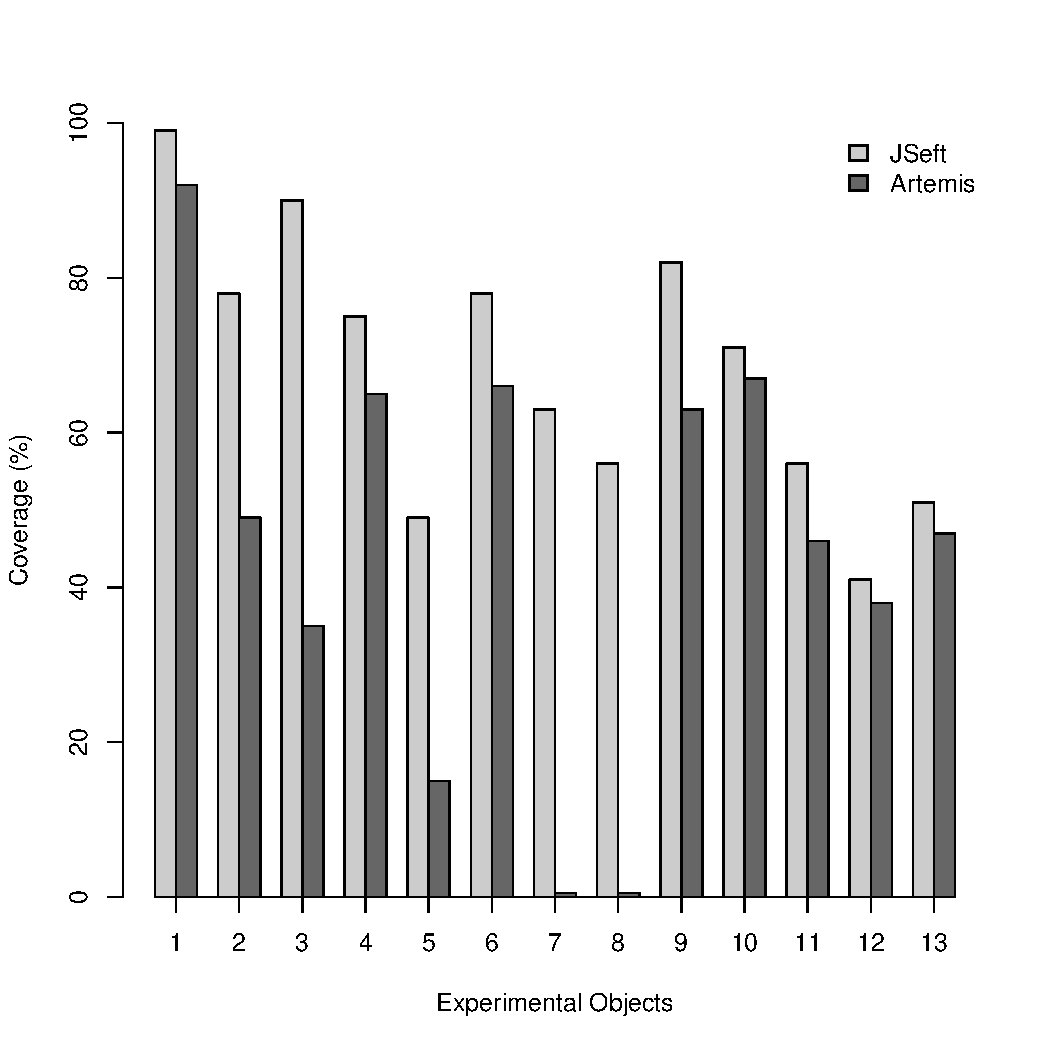
\includegraphics[width=1\hsize]{r-scripts/barplot_coverage}
  \vspace{-0.1in} 
  \mycaption{Statement coverage achieved.} 
  \vspace{-0.25in} 
  \label{Fig:coverage-graph}
\end{figure}


\headbf{Test Case Generation (RQ1)} 
\figref{coverage-graph} depicts the statement coverage achieved by \tool for each application. The results show that the test cases generated by \tool achieve a coverage of 68.4\% on average, ranging from 41\% (ID 12) up to 99\% (ID 1).
%\karthik{Do we need the text below ? We are better than random.}
We investigated why \tool has low coverage for some of the applications. For instance, we observed that in JointLondon (ID 7), the application contains \javascript functions that are browser/device specific, i.e., they are exclusively executed in Internet Explorer, or iDevices. As a result, we are unable to cover them using \tool. 
We also noticed that some applications required more time to achieve higher statement coverage (e.g., in NarrowDesign ID 8), or they have a large DOM state space (e.g., BunnyHunt ID 5) and hence \tool is only able to cover a portion of these applications in the limited time it had available.

\tabref{efficiency-abs-mut-table} columns under ``St. Coverage'' present \javascript statement coverage achieved by  our function coverage maximization algorithm versus a random strategy. The results show a 9\% improvement on average, for our algorithm, across all the applications. We observed that our technique achieves the highest improvement when there are many dynamically generated clickable DOM elements in the application, for example, GhostBusters (ID 3). 
%For instance, GhostBusters (ID 3) has 27\% more coverage since it contains a large number of dynamically created clickable DOM elements that appear and then disappear within a few seconds, which our technique can handle, but the random one may not. 
%We observed two anonymous functions, attached to clickable elements, that are missed by the random exploration technique in this application. Our technique is not only able to quickly spot such on the fly generated clickables, but it is also able to click on the ones that result in the execution of uncovered functions.

The columns under ``State Abstract'' in \tabref{efficiency-abs-mut-table} present the number of function states
before and after applying our function state abstraction algorithm.   
The results show that the abstraction strategy reduces function states by 85.5\% on average. NarrowDesign (ID 7) and FractalViewer (ID 9) benefit the most by a 97\% state reduction rate. 
%\karthik{What about ID 9 ?}
Note that despite this huge reduction, our state abstraction does not adversely influence the coverage as we include at least one function state from each of the covered branch sets as described in \secref{testCaseGen}.

The last two columns of \tabref{efficiency-abs-mut-table}, under ``Oracles'', present the number of assertions obtained by capturing the whole application's state,  without any mutations, and with our mutation-based oracle generation algorithm respectively. The results show that the number of assertions is decreased by 86.5\% on average due to 
our algorithm. 
We observe the most significant reduction of assertions for JointLondon (ID 7) from more than 198000 to 342. 
%\ali{by how much? what is the reduction rate?} 


%\ali{removing the insiginificant results} For example, for Tunnel (ID 2) and Fractal Viewer (ID 9), we observed no improvement in the statement coverage as these two applications have no dynamically generated or bound to event-listeners clickables. Instead, their few clickables are all placed in the HTML code of the application with a fixed event-handler per clikcable. Thus,  our approach achieves the same coverage as the random strategy for such applications.
%For SameGame (ID 1) the number of executed functions remains the same, for both approaches. However, in the limited five minute period of time, as a result of dynamically detecting valid clickable elements, \tool is able to examine different paths of the applications, while the random exploration technique fails to do so as it blindly clicks on any candidate element on the DOM tree.



%These two functions are attached to clickable elements that are not executed using random strategy.
%\figref{coverage-graph} presents our results for the statement coverage achieved by the test suite generated by \tool and \artemis. %The coverage is shown separately for the function-level unit tests and DOM event-based tests.     
%\tabref{efficiency-abs-mut-table} presents the number of function states
%before and after applying our function state abstraction mechanism.    
%The results show that the abstraction strategy is able to reduce the number of function states up to 97\%. NarrowDesign (id 7) with the largest
%number of function states benefits the most from our abstraction technique by 97\% state reduction. Note that we observed that our state abstraction does not affect the coverage. The reason is we select at least one function state from each of the covered branch sets as described in \secref{testCaseGen}.
%The last two columns of \tabref{efficiency-abs-mut-table} presents the number of all possible assertions obtained by capturing the whole application's state without performing any mutation, as well as the number of assertions after applying mutation. The results show that the number of assertions are drastically reduced by selectively pick only useful assertions during the mutation process.
% \tabref{testability-table} presents the testability of \javascript functions in the experimental objects.
% The table shows the total number of functions, number of functions that are testable, and the percentage of testable functions. 
% It also shows the number and the percentage of testable functions that are tested by the function-level tests generated by \tool (See Definitions \ref{testabilityFormula}-\ref{pythiaTestabilityFormula} in Section \ref{test-gen-setup}). 
% 
%As shown in \tabref{testability-table}, our generated function-level unit tests can, on average, examine 77\% of the testable functions. 
%This demonstrates the efficacy of our function covering technique in covering a considerable number of functions. 
%While \tool is able to examine up to 100\% of the testable functions for  SameGame, it can only cover 48\% of the testable functions for Fractal Viewer. 
%The low numbers for Fractal Viewer are mainly due to (1) the presence of random generator functions, and (2) the lack of support  for object input parameters with cyclic references in the current implementation of \tool, which we discuss in \secref{discussion}.

\begin{table}
%\vspace{5pt}
\centering
        \caption{Fault detection.}
        \label{Table:faultDetection-table}
{\scriptsize
       
      %  \subtable[Experimental subjects and the corresponding exploration data]
            {
           \begin{tabular}{c|c|rlllll||rr} \hline
& & \multicolumn{6}{c||}{\thead{\jseft}} & \multicolumn{2}{c}{\thead{\artemis}}\\
\cline{3-10}

\theadturn{App ID} &\theadturn{\# Injected Faults}
&\theadturn{\#FN} &\theadturn{\#FP} &\theadturn{\#TP} 
&\theadturn{Precision (\%)}  &\theadturn{Recall (\%)} & 
%\theadturn{$\frac{\#NotDetectedByEventTest}{\#TotalDetected}$(\%)} 
\theadturn{By func-level tests (\%)} 
&\theadturn{Precision (\%)} & \theadturn{Recall (\%)}  \\  \hline 

\hline

1  & 50 & 0 & 0 & 50 & 100 & 100 & 30 & 100 & 20  \\ 
           
2 & 50 & 9 & 0 & 41 & 100 & 82 & 73 & 100  & 12 \\ 

3 & 50 & 4 & 0 & 46 & 100 & 92 & 17 & 100 &  8 \\ 

4 & 50 & 15 & 0 & 35 & 100 & 70 & 28 & 100 & 22 \\ 

5 & 50 & 26 & 0 & 24 & 100 & 48 & 25 & 100 & 0 \\ 

6 & 50 & 9 & 0 & 41 & 100 & 82 & 15 & 100 &  16 \\ 

7 & 50 & 17 & 0 & 33 & 100 & 66 & 24 & 100 &  0%10
\\ 

8 & 50 & 23 & 0 & 27 & 100 & 54 & 26 & 100 &  0%6
 \\ 

9 & 50 & 6 & 0 & 44 & 100 & 88 & 41 & 100 &  24 \\ 

10 & 50 & 16 & 0 & 34 & 100 & 68 & 65 & 100 &  8 \\ 

11 & 50 & 21 & 0 & 29 & 100 & 58 & 27 & 100 &  6 \\ 

12 & 50 & 26 & 0 & 24 & 100 & 48 & 17 & 100 &  22 \\ 

13 & 50 & 23 & 0 & 27 & 100 & 54 & 26 & 100 &  28 \\ \hline

AVG & - & 15 & 0 & 35 & 100 & 70 & 32 & 100 & 12.8 \\ \hline

\hline\end{tabular}\centering
            }
} 
\vspace{-0.2in}
\end{table}
\headbf{Fault finding capability (RQ2)} \tabref{faultDetection-table} presents the results on the fault finding capabilities of \tool.
The table shows the total number of injected faults, the number of false negatives, false positives, true positives, and the precision and recall of \tool. 

\tool achieves 100\% precision, meaning that all the detected faults reported by \tool are real faults. {\em In other words, there are no false-positives.}
This is because the assertions generated by \tool are all stable \ie they do not change from one run to another. % as we do not observe any false positives. 
However, the recall of \tool is 70\% on average, and ranges from 48 to 100\%. This is due to false negatives, \ie missed faults by \tool, 
which occur when the injected fault falls is either in the uncovered region of the application, or is not properly captured by the generated oracles.  

%\begin{figure}[!t]
%  \centering
%  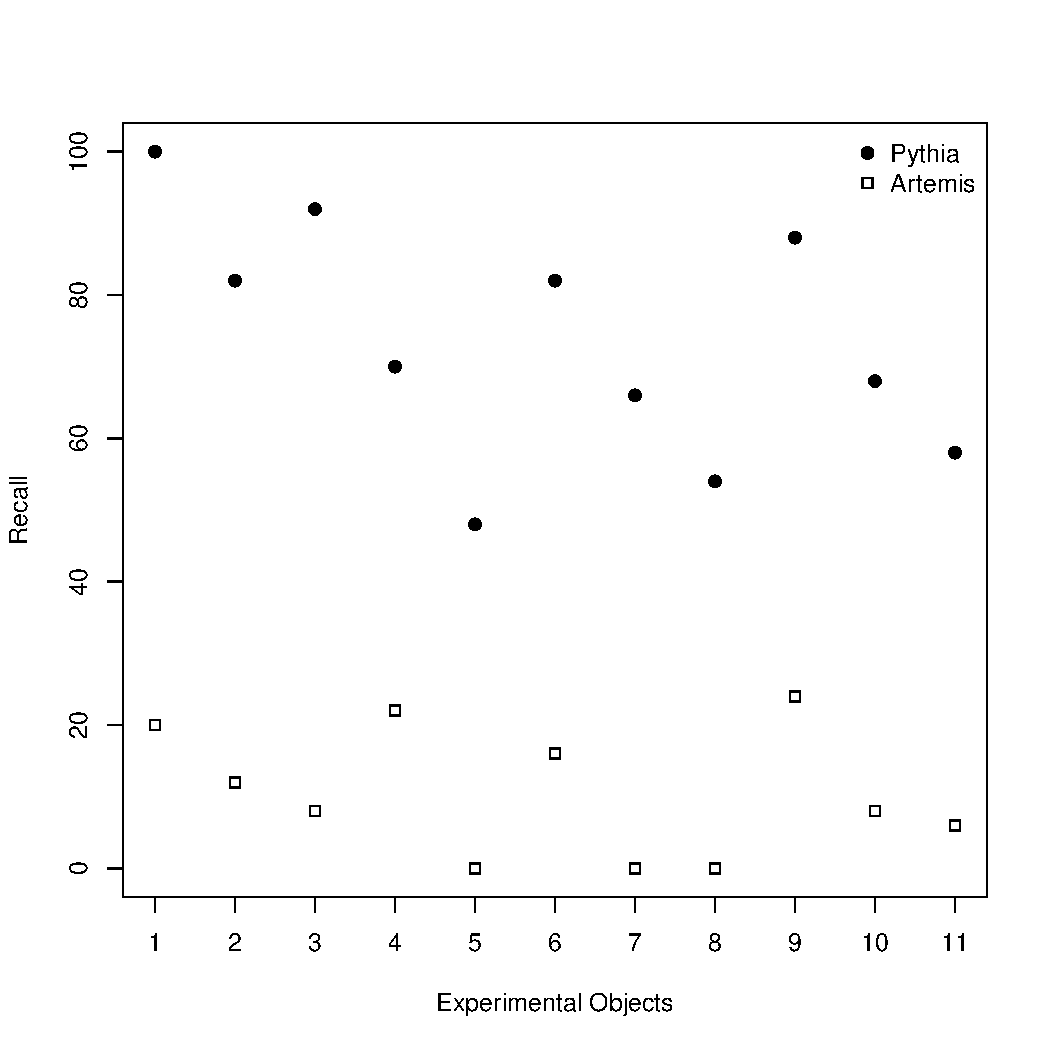
\includegraphics[width=0.9\hsize]{r-scripts/recall}
%  \mycaption{Recall of \tool and \artemis in detecting faults.}
%  \vspace{-0.1in} 
%  \label{Fig:recall-graph}
%\end{figure}

The table also shows that on average 32\% percent of the injected faults (ranges from 15--73\%) are detected by function-level test cases, but not by our DOM event-based test cases. This shows that a considerable number of faults do not propagate to observable DOM states, and thus cannot be captured by DOM-level event-based tests. 
For example in SimpleCart application (ID 10), if we mutate the mathematical operation that is responsible for computing the total amount of purchased items, the resulting error is not captured by event-based tests as the fault involves internal computations only. However, the fault is detected by a function-level test that directly checks the returned value of the function.
This points to the importance of incorporating function-level tests in addition to event-based tests for \javascript web applications. We also observed that even when an event-based test case detects a \javascript fault, localizing the error to the corresponding \javascript code can be quite challenging. However, function-level tests pinpoint the  corresponding function when an assertion fails, making it easier to localize the fault. 
%For example, in SameGame (ID 1), the function \code{compactDown} is responsible for moving cells up on the board after clicking on a given cell. If the index of the global variable \code{board} array is mutated in \code{compactDown}, the event-based tests shows an incorrect \code{background} value of the \code{css} property on the corresponding DOM elements. However, tracing the fault back to the responsible function is difficult. Using function-level tests, we can easily spot the assertion that is failed after calling \code{compactDown} function (e.g., \code{equal(board[3][4], 1)} failed).    

\headbf{Comparison (RQ3)}
\figref{coverage-graph} shows the code coverage achieved by  both \tool and \artemis on the experimental objects running for the same amount of time, \ie 10 minutes.
%Note that while \artemis only generates DOM event tests, \tool generates both unit tests and DOM event tests. 
%We compare the statement coverage achieved by \tool with that achieved by \artemis. 
The test cases generated by \tool achieve 68.4\% coverage on average (ranging from 41--99\%), while \artemis achieves only 44.8\% coverage on average (ranging from 0--92\%).
Overall, the test cases generated by \tool achieve 53\% more coverage than \artemis, which points to the effectiveness of \tool in generating high coverage test cases. 
Further, as can be seen in the bar plot of \figref{coverage-graph}, for all the applications, the test cases generated by \tool achieve higher coverage than those generated by \artemis. 
This increase was more than 226\% in the case of Bunnyhunt (ID 5). %\ali{Is this true? Isn't the difference in ID 7 and ID 8 more?}
For two of the applications, NarrowDesign (ID 7) and JointLondon (id 8), \artemis was not able to complete the testing task within the allocated time of ten minutes.
Thus we let \artemis run for an extra 10 minutes for these applications (\ie 20 minutes in total). Even then, neither application completes under \artemis. 
%By reducing the iteration option, \artemis produces an output after 10 minutes, however, with considerably lower coverage rates of 30\% and 35\% for NarrowDesign (ID 7), and JointLondon (ID  8), respectively. %I calculated the results based on zero coverage for these two apps, not sure if mentioning 30 and 35% here is correct or not!   

\tabref{faultDetection-table} shows the precision and recall achieved by \tool and \artemis.
With respect to fault finding capability, unlike \artemis that detects only generic faults such as runtime exceptions and W3C HTML validation errors, \tool is able to accurately distinguish faults at the code-level and DOM-level through the test oracles it generates. Both tools achieve 100\% precision, however, \tool achieves five-fold higher recall (70\% on average) compared with \artemis, which achieves 12.8\% recall on average. %Thus, \tool achieves more than five-fold increase in recall over \artemis.   

\subsection{Discussion} \label{Sec:discussion}
\begin{figure}[!t]
  \centering
  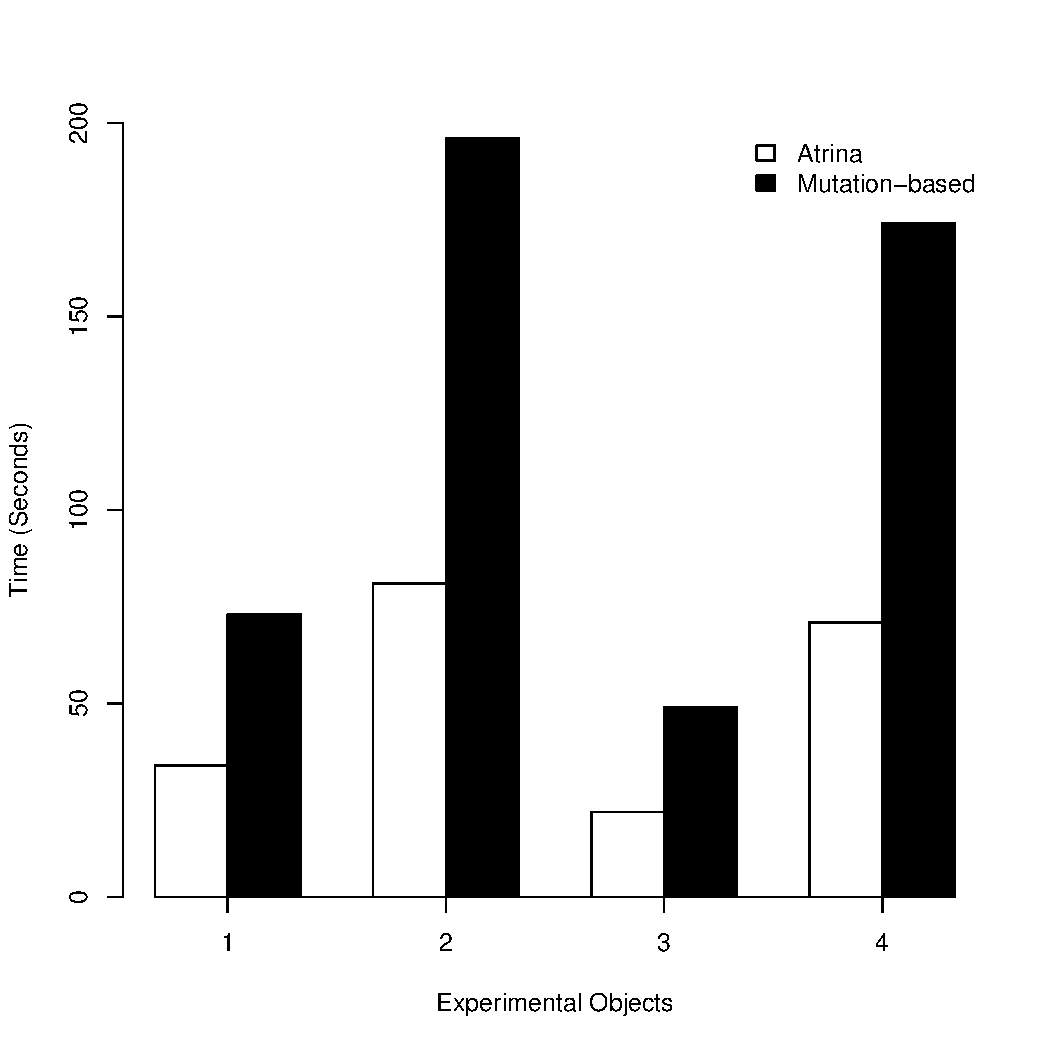
\includegraphics[width=0.7\hsize]{r-scripts/performance}
  \vspace{-0.18in}   
  \mycaption{Time overhead for each approach.}
  \vspace{-0.3in} 
  \label{Fig:performance}   
\end{figure}
% Moved time efficiency to results
%Moreover, this reiterates the known performance shortcomings of approaches that rely on mutant generation.
\headbf{Fault Masking} As we mentioned in \secref{explicitAssertions}, the concrete value of an entity in the computed backward slice can potentially be used as the expected value of the entity in explicit assertions to test the current version of the application.
The actual values of the related entities in the backward slice are correct unless there exists a masked fault which is concealed in the chain of computations and thus does not propagate to the checked state of the DOM element. However, we conjecture that fault masking rarely happens in \javascript web applications as it is more prevalent in programs with many small expressions whose results are stored in several intermediate values. We also observed no fault masking occurrence during the evaluation of \tool on seven \javascript applications used in this study.
\headbf{Limitations} The effectiveness of the generated assertions by \tool in terms of fault finding capability depends on the quality of human-written DOM-based test cases. If the DOM assertions contained in the DOM-based test suite check irrelevant information, the explicit assertions obtained by our tool will point to entities that may not be important from the tester's point of view. This can also negatively affect the fault finding capability of implicit assertions as they are indirectly inferred from the DOM-based assertions. Moreover, if the human-written test suite does not execute application's state with effective DOM elements, our tool is not able to infer effective candidate assertions.   
\subsection{Threats to Validity} \label{Sec:threatsToValidity}
An external threat to the validity of our evaluation is the limited number of \javascript applications used to measure the effectiveness of our approach. We mitigated this threat by using web applications from various domains, code size, and functionality. Another threat concerns validating failed assertions through manual inspection that can be error-prone. To mitigate this threat, we carefully examine the code in which the assertion failed to make sure that the injected fault was indeed responsible for the assertion failure. Moreover, manual computation of the \javascript slices to measure precision and recall is a time intensive task done by the authors of the paper, and thus could be error-prone. However, we made every effort to mitigate this threat by precisely examining the application's code.

The regression faults we inject to evaluate the effectiveness of \tool may not be realistic. We mitigate this threat by injecting mutations that represent common \javascript applications faults, as well as using real-world web applications, and \selenium test cases written by developers. 

